\documentclass{article}
\usepackage[utf8]{inputenc}
\usepackage{natbib}
\usepackage{graphicx}
\usepackage{subfigure}
\usepackage{amssymb}
\usepackage{amsmath}
\usepackage{amsthm}
\usepackage{mathtools}
\usepackage{mathrsfs}
\usepackage{epstopdf}
\usepackage{booktabs}
\usepackage{setspace}
\usepackage{cases}
\usepackage{dsfont}
\usepackage{algorithm}
\usepackage{algorithmicx}
\usepackage{algpseudocode}
\usepackage[colorlinks,linkcolor=blue,anchorcolor=blue,citecolor=blue,urlcolor=blue]{hyperref}

\usepackage{tikz}
\usepackage{forest}

\usepackage[left=1in,right=1in,top=1in,bottom=1in]{geometry}

\newtheorem{example}{Ex}[section]
\newtheorem{defn}{Def}[section]
\newtheorem{thm}{Theorem}[section]
\newtheorem{col}{Corollary}[section]
\newtheorem{rem}{Rmk}[section]
\newtheorem{lem}{Lemma}[section]

\usepackage{color}
\definecolor{backcolor}{rgb}{0.6,0.6,0.6}
\pagecolor{backcolor}

\title{ Game Project }
\author{Yixiang Luo, Qi Huang, Yahui Cui }
\date{\today}

\renewcommand{\baselinestretch}{1.5}
\newcommand{\book}[1]{\textit{#1}}
\newcommand{\C}{\textbf{Comments:}}
\newcommand{\Q}{\textbf{Questions:}}
\newcommand{\pth}[1]{\left( #1 \right)}
\newcommand{\br}[1]{\left[ #1 \right]}
\newcommand{\cur}[1]{\left \{  #1 \right \}}
\newcommand{\vct}[1]{\boldsymbol{#1}}
\newcommand{\mat}[1]{\boldsymbol{#1}}
\newcommand{\abs}[1]{| #1 |}
\newcommand{\norm}[1]{|| #1 ||}
\newcommand{\set}[1]{\left \{  #1 \right \}}
\newcommand{\mon}[1]{\left \langle #1 \right \rangle}
\newcommand{\Rset}{\mathbb{R}}
\newcommand{\pt}[1]{\dot{#1}}


\begin{document}

\maketitle

\begin{spacing}{1.4}

\section{Experiment Result and Analysis}
\subsection{Result: trend of the game value}
We conducted $t$ times experiments for each $n \in [1,20]$, computed and plotted the mean and variance of the game value for each $n$, where $n$ is the total steps of our game. \newline
By taking a look at the original data, we first noticed the relationship between $n$ and the mean value. In Fig. 1, we found the mean of game value fluctuates in a zigzag version with the increasing of $n$. Because Paul always play at first, the game value goes down from $n=1$ to $n=2$. Assuming we are at $n=i$, if mean value goes up from $i-1$ to $i$, then it goes down from $i$ to $i+1$ and vice versa. If we looked at the range of value and the corresponding n more precisely, we found that with $n$ increasing,the mean of value fluctuates in a constant range with changing between positive and negative. In addition, when $n$ is odd, the mean value is always positive and goes to negative in the next time; if n is even, the value is negative and will become positive later. Besides, the mean never goes to zero, indicating there is advantage in this game.\newline
Our next observation focused on the variance of experiments for each $n$. With the same sample number for every $n$, however, we found the variance of the sampled game value decreasing rapidly with the increasing of n. It starts from 0.15 and converges to 0. The convergence of sample variance has no relationship with the parity of $n$.\newline
Our observations on mean and variance of the sampled game value motivated us to search the game value in the way below:\newline
\begin{enumerate}
    \item The relationship between parity of $n$ and the mean of game value suggests us to study the game value in two cases separately. We will study the trend of the mean game value when $n$ is even and when $n$ is odd. This is reasonable as we know when $n$ is odd, Paul will play the last step and has control of the final result by choosing the maximum value of all leaves; while when $n$ is even, Carol will play the last step by choosing the minimal value of all leaves and the only thing for Paul is to receive the game result. That is to say, the advantage comes in the last step.
    \item The change of variance is a little bit amazing to us, which implies that in either case, the game value may converge with the increasing of $n$, regardless to the parity of $n$.
    \item Together with the two points above, we infer that the game value might converge to two different points when goes to infinity and the points depend on the parity of $n$(the point is different when $n$ is odd and even).
\end{enumerate}
To verify our assumption, we first study the distribution of the sampled game value for different $n$. We skipped the first several $n$ and plotted the experiment results in two groups: one is that $n$ is even, other is that $n$ is odd.\newline
We plot the histograms of the sampled game value and normed the graph so that the sum of the area of each bin is 1. The x-axis is the value while y-axis denotes the probability density of the corresponding score. We denote $(a_i,b_i)$ is the $i_{th}$ bin of the histogram, $N_i$ is the number of sample in that bin and $N$ is the number of samples for each $n$ and normed the graph in the way below, where $p(value=X)$ is the probability density of value when $value = X$:
\begin{equation*}
    P(X \in (a_i,b_i)) = \frac{N_i}{N}
\end{equation*}
\begin{equation*}
    p(value = X, X \in (a_i,b_i)) = \frac{P(X \in (a_i,b_i))}{(b_i,a_i)}
\end{equation*}
Fig 2. shows the odd case of $n$ with $n=13,15,17,19$. From Fig 2., we observed that the distribution of sampled game value in each subplot forms a normal distribution asymptotically, centering around the mean of that sample. When $n$ increases, the distribution shrinks to the corresponding center, which verifies the decreasing variance when $n$ increases. The center for each distribution, however, also converges to some point between $(0.20,0.30)$.\newline
Fig 3. represents the case when $n$ is even, where $n = 14, 16, 18, 20$. The change of the distribution is similar to the case when $n$ is odd except that the center for each distribution converges to some point in $(-0.25, -0.15)$. \newline

\subsection{Data Analysis}
By now, we have discovered that the game value converges when $n$ goes to infinity, but the value converged to is different between cases when $n$ is odd and even. We will then present more details on how game value converges and the properties of the points which the value converges to.\newline
Fig 5. shows a more clear trend for the distribution of game value under different $n$. With y-axis representing the probability density estimated from the histograms, all red lines denote the game value distribution when $n$ is odd, while all green lines represent that when $n$ is even. For all the red lines, we could see while the center of each distribution converges to one point in $(0.20,0.30)$, the peak of each distribution increases rapidly. This implies that the density of the center increases quickly with the increasing of $n$. Denote the point which the game value converges to when $n$ is odd as $X_{odd}$, the trend also shows suggests that the probability density of $X_{even}$ goes to infinity. The trend for distribution of game value when $n$ is even is rather similar. With the fast increasing of the peak of the distribution, the center of all distribution converges to a point $X_{even}$ in $(-0.25, -0.15)$\newline
Besides the convergence, we also want to find some properties of the two points, $X_{odd}$ and $X_even$. To do that, we first estimated the points which value converges to with n in different parity. We take several value of $n$ and found the bin (denoted by the corresponding interval $(a_i, b_i)$) with the maximum area, meaning the probability of game value drops in that bin is highest among all bins. Then, we take the average of the endpoints of that interval as our estimator for the converges point of each $n$. As we know the range of game value is $[-1,1]$, we then want to find the relationships between the points and the game value. Figure 6 and Figure 7. present our estimated probability density for the middle point of each bin with $n$ in odd and even respectively with confidence interval. Table 1. shows our estimates of the converge points for each $n$. In Table 1., we also calculated the relative position of the converge point in the range of game value and the ratio of distances for the point to the middle of the game value range. We denote $d_{odd}$ to be the relative position of $X_{odd}$, $d_{even}$ to be the relative position of $X_{even}$, $[a,b]$ to be the range of the game value, $M$ to be the middle of the range and $r$ to be the ratio of $|X_{odd}-M|$ and $|X_{even}-M|$. We define $d_{odd}$, $d_{even}$ and $r$:
\begin{equation*}
    d_{odd}=\frac{|X_{odd}-a|}{|b-a|} \quad d_{even}=\frac{|X_{even}-a|}{|b-a|}
\end{equation*}

\begin{equation*}
    r = \frac{|X_{odd}-M|}{|X_{even}-M|}
\end{equation*}
\subsection{Verification}
In the next part, we will present the theoretical analysis of the distribution of the game value. Here, we show the result of our experiment with the theoretical results.


\section{Theory Analysis}
\subsection{Recurrence relation}
A typical structure of the game looks like the follows.
\begin{center}
  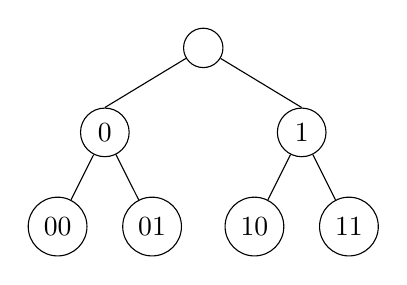
\begin{tikzpicture}[
    node/.style={circle, draw, rounded corners=1mm, text centered, anchor=north, text=black, minimum size=5mm},
    empty/.style={circle, draw=none, text centered, anchor=north, text=black, size=5mm},
    level distance=0.5cm,
    growth parent anchor=south,
    ]
      \node [node] {$~$}
      [sibling distance=2.5cm]
      child{ [sibling distance=1.2cm]
        node [node] (a) {$0$}
        child{
          node [node] {$00$}
        }
        child{
          node [node] {$01$}
        }
      }
      child{ [sibling distance=1.2cm]
        node [node] (a) {$1$}
        child{
          node [node] {$10$}
        }
        child{
          node [node] {$11$}
        }
      };
  \end{tikzpicture}
\end{center}

Each node has a value and it is a random variable. It is easy to show that if the values of all leaf nodes are i.i.d., the values of nodes having the same height are also i.i.d. Assume the leaf nodes have height $0$ and denote the cumulative distribution function (CDF) of the values on nodes having height $i$ as $F_i(x)$, and the corresponding random variable as $V_i$. In the algorithm, the value of a internal node is calculated by taking the maximum or minimum of its two children. So we have
\begin{equation}
  \left\{
  \begin{array}{ll}
    F_{i+1} = F_i^2, & \text{ if take maximum}\\
    F_{i+1} = 1 - (1 - F_i)^2 = 2 F_i - F_i^2, & \text{ if take minimum}
  \end{array}\right.
\end{equation}
Combining the order of playing of the game, we conclude that
\begin{equation}
  \left\{
  \begin{array}{ll}
    F_{i+1} = F_i^2, & \text{ if $i+n$ odd, $i \leq n-1$}\\
    F_{i+1} = 1 - (1 - F_i)^2 = F_i (2 - F_i), & \text{ if $i+n$ even, $i \leq n-1$}
  \end{array}\right.
\end{equation}

\subsection{Convergence}
Now let's combine two successive updates and derive the relationship as follows.
\begin{numcases}{}
  F_{i+2} = L(F_i) \equiv F_i^2 (2 - F_i)^2, & \text{ if $i+n$ even, $i \leq n-2$} \label{two_step} \\
  F_{1} = F_0^2, & \text{ if $n$ odd} \label{init_ts}
\end{numcases}
What we concern about is the value of the root node, i.e. $F_n$. And the reccurence above is enough for this purpose. If $n$ is even, we apply (\ref{two_step}) on $F_0$ and finally we will reach $F_n$. If $n$ is odd, we apply (\ref{init_ts}) on $F_0$ and then (\ref{two_step}) and finally we will also reach $F_n$.

Now we can state our main result.

\begin{thm} \label{convergence}
The CDF of the value of the root node, i.e. $F_n$, converges pointwisely on even $n$ or odd $n$ sequence. Specifically,
\begin{enumerate}
  \item for even $n$, $F_n$ converge to $\mathds{1}_{x \geq x_1}$, where $F_0(x_1) = 1 - \phi$;
  \item for odd $n$, $F_n$ converge to $\mathds{1}_{x \geq x_2}$, where $F_1(x_2) = F_0^2(x_2) = 1 - \phi$;
\end{enumerate}
where $\mathds{1}$ is the indicator function and $\phi = \frac{\sqrt{5}-1}{2}$ is the Golden ratio.
\end{thm}

\begin{proof}
  \begin{enumerate}
    \item Since $n$ is an even number, after applying $n/2$ times of reccurence (\ref{two_step}) on $F_0$ we get $F_n$. Now let's look at the difference after one reccurence
    \begin{equation}
      D(F_i) = F_{i+2} - F_i = L(F_i) - F_i = F_i^2 (2 - F_i)^2 - F_i
    \end{equation}
    For simplicity, let's ignore the subscript and simply write
    \begin{equation}
      D(F) = F^2 (2 - F)^2 - F.
    \end{equation}
    The function $D(F)$ has only three zeros in $[0, 1]$, which are
    \begin{equation}
      0, \quad 1 - \phi, \quad 1,
    \end{equation}
    and its graph is shown in Figure \ref{D_F}.
    \begin{figure}[!htb] \centering
      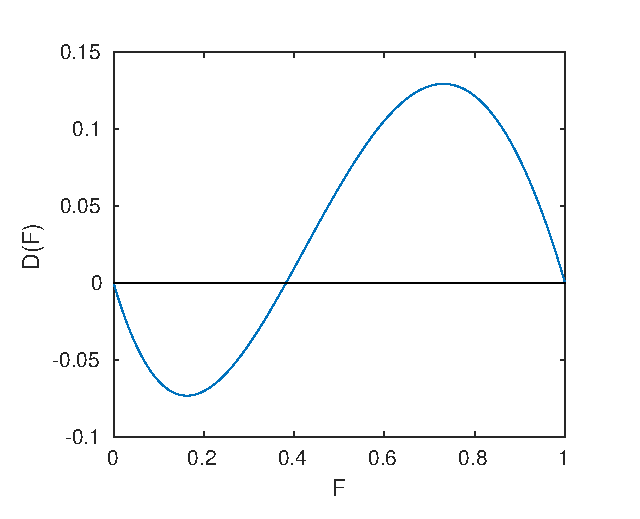
\includegraphics[width=0.4\columnwidth]{figures/D_F.eps}
      \caption{The graph of $D(F)$.}
      \label{D_F}
    \end{figure}

    If $F > 1 - \phi$, after applying the operator $L$ on F, $L(F) > F > 1 - \phi$. So $L^k (F)$ is a strictly increasing function of $k$, if $F > 1 - \phi$, where $L^k (F)$ means applying the operator $L$ $k$ time. In addition, since $L^k (F)$ is a restriction of the CDF $F_{2k}$, we have $L^k (F) \leq 1$. Therefore $F_{2k}(x) \; (F_0(x) > 1 - \phi)$ converges as $k$ goes to infinity.
    Moreover, since there is only one zero of $D(F)$ in $(1 - \phi, 1]$, which is $1$, the only stationary point of $L(F)$ in $(1 - \phi, 1]$ is $1$. Thus $F_{2k}(x) \; (F_0(x) > 1 - \phi)$ converges to $1$.

    Similarly, we have $F_{2k}(x) \; (F_0(x) < 1 - \phi)$ converges to $0$.

    Combining all above, we conclude
    \begin{equation}
      F_n(x) \to \mathds{1}_{F_0(x) \geq 1 - \phi}, \text{ as } n \to \infty, \quad \text{$n$ even}
    \end{equation}

    \item When $n$ is odd, applying the same analysis, but notice now the initial value of the reccurence (\ref{two_step}) is $F_1$, we derive
    \begin{equation}
      F_n(x) \to \mathds{1}_{F_1(x) \geq 1 - \phi} \equiv \mathds{1}_{F_0^2(x) \geq 1 - \phi}, \text{ as } n \to \infty, \quad \text{$n$ odd}
    \end{equation}

  \end{enumerate}
\end{proof}

Then we have the following corollaries immediately.
\begin{col}
  Denote the probability distribution function corresponding to $F_n(x)$ as $f_n(x)$. Then
  \begin{enumerate}
    \item for even $n$, $f_n$ converge to $\delta(x - x_1)$, where $F_0(x_1) = 1 - \phi$;
    \item for odd $n$, $F_n$ converge to $\delta(x - x_2)$, where $F_1(x_2) = F_0^2(x_2) = 1 - \phi$;
  \end{enumerate}
  where $\delta(x)$ is the Dirac delta function.
\end{col}

\begin{col} Denote $\mathbb{E} (V_n)$ and $var(V_n)$ as the expectation and variance of $V_n$ respectively.
  \begin{enumerate}
    \item For even $n$, $\mathbb{E} (V_n) \to x_1$ and $var(V_n) \to 0$, where $F_0(x_1) = 1 - \phi$.
    \item For odd $n$, $\mathbb{E} (V_n) \to x_2$ and $var(V_n) \to 0$, where $F_1(x_2) = F_0^2(x_2) = 1 - \phi$.
  \end{enumerate}
\end{col}

\subsection{Uniform distribution}
Assume $V_0 \sim U([0, 1])$. Now $F_0(x) = x$ and $F_1(x) = x^2$ ($n$ odd). So
\begin{equation}
  x_1 = 1 - \phi, \quad x_2 = \phi
\end{equation}
and
\begin{enumerate}
  \item For even $n$, $\mathbb{E} (V_n) \to 1 - \phi \approx 0.382$ and $var(V_n) \to 0$.
  \item For odd $n$, $\mathbb{E} (V_n) \to \phi \approx 0.618$ and $var(V_n) \to 0$.
\end{enumerate}

\subsection{Pseudocode}
\begin{algorithm}[htb!] \label{Num-DLCS}
  \caption{Num-DLCS}
  \begin{algorithmic}[1] %每行显示行号

    \Require sequence $X_m$, $Y_n$.
    \Ensure the number of the distinct longest common subsequences in $(X_m, Y_n)$.

    \Function {Num-DLCS}{$X_m, Y_n$}
      \State $S(i,0) = [1, 0, 0, \cdots, 0] \in \Rset^{1 \times (\max(m,n)+1)}$ ~~\textbf{for} $i=0, \cdots, m$
      \State $S(0,j) = [1, 0, 0, \cdots, 0] \in \Rset^{1 \times (\max(m,n)+1)}$ ~~\textbf{for} $j=0, \cdots, n$
      \For {$i$=1; $i \leq m$; $i$++}
        \For {$j$=1; $j \leq n$; $j$++}
          \If{$X(i)$ == $Y(j)$}
            \State $p$ = largest index of element of $X_{i-1}$ satisfying $X(p)$==$X(i)$
            \State $q$ = largest index of element of $Y_{j-1}$ satisfying $Y(q)$==$Y(j)$
            \State $S(i,j) = S(i-1,j-1) + \text{MoveRight}(S(i-1,j-1)) - \text{MoveRight}(S(p-1,q-1))$
          \Else
            \State $S(i,j) = S(i,j-1) + S(i-1,j) - S(i-1,j-1)$
          \EndIf
        \EndFor
      \EndFor
      \State \Return the last nonzero element of $S(m,n)$
    \EndFunction

  \end{algorithmic}
\end{algorithm}


\end{spacing}
\end{document}
